¿Cuál es el área del triángulo rectángulo de la figura \ref{fig:area_rectangulo_01}?

\begin{figure}[H]
    \begin{center}
        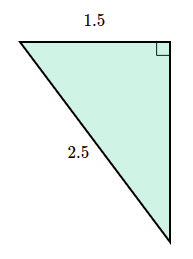
\includegraphics[width=0.15\linewidth]{../images/area_rectangulo_01.png}
    \end{center}
    \caption{}
    \label{fig:area_rectangulo_01}
\end{figure}
\begin{solutionbox}{14cm}

    \begin{minipage}{0.6\textwidth}
        Para determinar el área del triángulo debemos saber la base y la altura. Llamemos $x$ a la longitud (ver Figura \ref{fig:area_rectangulo_01a}).
        Cuando tenemos un triángulo rectángulo, podemos usar el teorema de Pitágoras para obtener la longitud del cateto.
        La ecuación para el teorema de Pitágoras es:
        \[c^2=a^2+b^2\]
        En este caso, $a=1.5$, $b=x$ y $c=2.5$, Entonces,
        \begin{align*}
            1.5^2+x^2 & =2.5^2     \\
            2.25+x^2  & =6.25      \\
            x^2       & =6.25-2.25 \\
            x^2       & =4         \\
            x         & =2
        \end{align*}
        La altura del triángulo es 2. El área del triángulo es:

        \begin{align*}
            A & =\frac{1}{2}bx               \\
            A & =\frac{1}{2}\cdot 1.5\cdot 2 \\
            A & =1.5 \text{ u}^2
        \end{align*}
    \end{minipage}\hfill
    \begin{minipage}{0.35\textwidth}
        \begin{figure}[H]
            \centering
            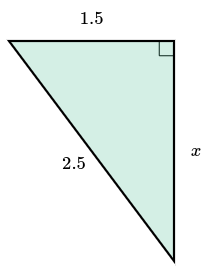
\includegraphics[width=0.5\linewidth]{../images/area_rectangulo_01a.png}
            \caption{}
            \label{fig:area_rectangulo_01a}
        \end{figure}
    \end{minipage}

\end{solutionbox}

